\documentclass[12pt]{exam}

\usepackage{graphicx} % allows for graphics
\usepackage{ifthen}  % for if statements 

\newcommand{\sol}{1} %solution =1 or 0

% LOAD PACKAGES
\usepackage{amsmath} % allows for align env and other things
\usepackage{amssymb} % 
\usepackage{mathtools} % allows for single apostrophe
\usepackage{enumitem} % allows for alpha lettering in enumerated lists
\usepackage{lastpage}
\usepackage{array} % for table alignments
\usepackage{graphicx} % if images are needed

\addpoints

\usepackage{pgfplots} % for surfaces (chapter 7)
\usepackage{tikz-3dplot} 
\pgfplotsset{compat=1.9}
\usetikzlibrary{decorations.pathmorphing,patterns} % for some tikz diagrams
% ~~~~~~~~~~~~~~~~~~~~~~~~~~~~~~~~~~~~
% INITIALS
\newcommand{\Initials}{\textit{\Course, \TestName. Your initials: \underline{\hspace{3cm}}} \vspace{1pt}}

\newcommand{\InitialsLeft}{\noindent \hspace{-18pt}\textit{\Course, \TestName. Your initials: \underline{\hspace{3cm}}} \vspace{1pt}}

\newcommand{\InitialsRight}{\begin{flushright}\textit{\Course, \TestName. Your initials: \underline{\hspace{3cm}}} \vspace{1pt}\end{flushright}}

% ~~~~~~~~~~~~~~~~~~~~~~~~~~~~~~~~~~~~
% INSTRUCTIONS FOR DISTANCE LEARNING WITH NO PROCTOR
\newcommand{\InstructionsFormatAndTiming}{

    \begin{itemize} \setlength\itemsep{.1em}
    
        % \item You should only need 75 min to take the exam, but students will have \Duration to submit the exam, from the time that it is released.
        
        \item {\bf Show your work} and justify your answers for all questions unless stated otherwise.
        
        \item Please write neatly, and use dark and clear writing so that the scan is easy to read. 
        
        \item Please write your name or initials at the top of every page 
        
        \item Please solve the questions in the exam in the order they are given. 
        
        \item You do not need to print the exam. As long as you solve problems in the order they are given (just like the written homework sets), you can write your answers on your own paper. But students can print the exam and write their answers on the printed copy if they prefer. 
        
    \end{itemize}

}

\newcommand{\InstructionsSubmission}{

    \begin{itemize} \setlength\itemsep{.1em}
        \item Students should scan their work and submit it through Gradescope. There should be an \textbf{assignment} in Gradescope for this exam. The process for submitting your work will be similar to what you have used for homework. 
        
        \item Work must be submitted by \DueDate. 
        
        \item Please upload your work as a single PDF file. If this is not possible you can email your work to your instructor. 
        
        \item During the upload process in Gradescope, please indicate which page of your work corresponds to each question in the exam. 
    \end{itemize}
}

\newcommand{\InstructionsQuestions}{

    \begin{itemize} \setlength\itemsep{.1em}
        
        \item If there are questions during the exam, students can email their instructor or message them through Canvas. 
        
        \item Our course Piazza forum will be temporarily inactive during the exam. 
        
        \item If you run into any technical issues or any unanticipated emergencies, please email your instructor as soon as you can. 
    
        
    \end{itemize}

}


\newcommand{\InstructionsHonor}{

    \begin{itemize} \setlength\itemsep{.1em}    
        \item Students can use any resources while taking these tests including online calculators and Mathematica
        \item Students cannot communicate with anyone during these tests.
        \item Students cannot use solutions provided from another student or third party. 
        \item In other words: do your own work but you can use technology to solve problems. 
 
    \end{itemize}

}






\newcommand{\GTHonorCode}{Having read the Georgia Institute of Technology Academic Honor Code, I understand and accept my responsibility as a member of the Georgia Tech community to uphold the Honor Code at all times. }



% FANCY HEADERS - MAKE EMPTY
\pagestyle{headandfoot}
\runningfooter{}{}{}


% ADJUST MARGINS FOR DISTANCE LEARNING REQUIREMENTS
\usepackage[tmargin=1.0in,bmargin=1.0in,left=1in,right=1in]{geometry}


% TIKZ DIAGRAMS
\usepackage{color}
\usepackage{tikz}  \usetikzlibrary{arrows} 
\usetikzlibrary{calc} 


% ADJUST FIRST LINE IN PARAGRAPH INDENTATION 
\setlength\parindent{0pt}


% COURSE SPECIFIC INFORMATION
\newcommand{\Course}{Math 2552}
\newcommand{\Instructors}{}

% WHO TO CONTACT DURING EXAM IF QUESTIONS
\newcommand{\InstructorContact}{}

\usepackage{spalign} % Joe Rabinoff's matrix package

\newcommand{\LastPage}{\begin{center}\textit{This page may be used for scratch work. Please indicate clearly if you would like your work on this page to be graded. }\end{center}   }


% DERIVATIVES
\newcommand{\dydt}{{\frac{dy}{dt}}} % 
\newcommand{\dydx}{{\frac{dy}{dx}}} % 
\newcommand{\dydtt}{{\frac{d ^2y}{dt^2}}} % 
\newcommand{\dydxx}{{\frac{d^2y}{dx^2}}} % 
\newcommand{\dydttt}{{\frac{d^3y}{dt^3}}} % 

\newcommand{\ddt}{{\frac{d}{dt}}} % 
\newcommand{\ddx}{{\frac{d}{dx}}} % 
\newcommand{\dudt}{{\frac{du}{dt}}} % 
\newcommand{\dvdx}{{\frac{dv}{dx}}} % 
\newcommand{\dxdt}{{\frac{dx}{dt}}} % 
\newcommand{\dxdtt}{{\frac{d^2x}{dt^2}}} % 
\newcommand{\dzdt}{{\frac{dz}{dt}}} % 



% COLORS FOR DIAGRAMS
\definecolor{DarkBlue}{rgb}{0.0,0.0,0.6} % 
% \definecolor{DarkGreen}{rgb}{0.0,0.3,0.0} % 
% \definecolor{DarkRed}{rgb}{0.6,0.0,0.0} % 

% TEST SPECIFIC INFORMATION
\newcommand{\TestName}{Sample Midterm 1}
\newcommand{\TestTime}{}
\newcommand{\Duration}{3 hours }
\newcommand{\Points}{}
\newcommand{\DueDate}{12:30 PM ET}


% \usepackage{tikz}
% \usetikzlibrary{shapes,snakes}   
% \usetikzlibrary{arrows,automata}

\begin{document}
    

\vspace*{-1cm}

\begin{center}
{\Large \TestName, \Course }
\end{center}

% \begin{center}    
% {\small
% Instructor: \Instructors \\ Administered on \TestDate. Students should have 3 hours to take this exam. 
% }
% \end{center}


% INSTRUCTIONS FOR STUDENTS
\vspace{2pt}
\begin{center}\textbf{{\large Instructions (PLEASE READ)}}\end{center}
\textbf{Formatting and Timing}
{\small \InstructionsFormatAndTiming}
\textbf{Submission}
{\small \InstructionsSubmission}
\textbf{Questions}
{\small \InstructionsQuestions}
\textbf{Integrity}
{\small \InstructionsHonor}

 % cover page for unproctored exam

\newpage

\begin{questions}

%  ~ ~ ~ ~  ~ ~ ~ ~  ~ ~ ~ ~  ~ ~ ~ ~  ~ ~ ~ ~  ~ ~ ~ ~
 
\question[10] Solve the following initial value problems. You may leave your answers as implicit relations in $t$ and $y$. 

    \begin{parts} 
    
        \part $\displaystyle y\dydt = (t + ty^2)e^{t^2}, \quad y(0) = 2$
        \part $\displaystyle t^3 \dydt + 4t^2 y = e^{-t}, \quad t < 0, \quad y(-1) = 0$
        
    \end{parts}

    \ifnum \sol=1
        {\color{DarkBlue} \textbf{Solution}\\ 
        \begin{enumerate}
            \item[a)] This question based on 2.1 \# 7. Separable: 
        \begin{align*}
            \frac{y}{1+y^2} dy &= te^{t^2} dt \\
            \int \frac{y}{1+y^2} dy &= \int te^{t^2} dt + C, \quad \text{set } u = t^2, du = 2t dt \\
            \frac12 \ln (1+y^2) &= \frac12 \int e^u du + C \\
             \ln (1+y^2) &= e^{t^2} + C \\
            y(0) = 2: \quad \ln (1 + 2) &= e^0 + C \quad \Rightarrow \quad C = \ln 3 - e \\
            \ln( 1 + y^2) &= e^{t^2} + \ln 3 - e
        \end{align*}
        
        \item[b)] This is question 2.2 \#19. If you have been working through the recommended homework exercises you should have the solution. The solution to the differential equation with arbitrary constant $c_1$ is $$y = c_1t^{-4} - t^{-4} e^{-t} - t^{-3}e^{-t}$$
        We were given that $y(-1) = 0$, so
        \begin{align*}
            0 &= c_1(-1)^{-4} - (-1)^{-4} e^{1} - (-1)^{-3}e^{1} \\
            0 &= c_1 - e + e \\
            c_1 &= 0
        \end{align*}
        The solution to the initial value problem (IVP) is
        $$y = - t^{-4} e^{-t} - t^{-3}e^{-t}$$
        
        \end{enumerate}
        
        }
    \fi 
    
\newpage\Initials

\question[10] Suppose $A = \spalignmat{-3 2; 1 1}.$  % based on 3.4 # 10
 	
  \begin{parts} 
    
        \part Determine the eigenvalues of $A$. Show your work. 
        \part Determine the eigenvectors of $A$. Show your work.
        \part Express the general solution of the system $\vec x \, ' = A \vec x$ in terms of real valued functions. Show your work. 
        \part Sketch the phase portrait of the system. Show your work.      
        
    \end{parts}
    
    
    \ifnum \sol=1
    {\color{DarkBlue} \textbf{Solution}
    
            \begin{enumerate}[label=(\alph*)]
        \item Characteristic polynomial: 
        \begin{align*}
            0 &= (-3 - \lambda) (1 - \lambda) - 2 \\
            &= \lambda^2 +2\lambda - 5 \\
            \lambda &= -1 \pm \frac12 \sqrt{4+20} = -1 \pm \sqrt{6}
        \end{align*}
        \item Eigenvectors: 
        \begin{align*}
            A - (-1 \pm \sqrt{6}) I = \begin{pmatrix} -2\mp\sqrt{6} & 2 \\ \ast & \ast \end{pmatrix}
        \end{align*}
        $\ast$ = not needed because $A-\lambda I$ is singular. The first row gives us $(-2 \mp \sqrt6)x_1 + 2x_2 = 0$. If $x_1 = 2$, then $x_2 = 2 \pm \sqrt6$. Eigenvectors are: 
        $$\vec v_1 = \spalignmat{2;2+\sqrt6}, \quad \vec v_2 = \spalignmat{2;2-\sqrt6}$$
        \item $\displaystyle \vec x(t) = c_1 e^{(-1+\sqrt6) t}\spalignmat{2;2+\sqrt6} + c_2e^{(-1-\sqrt6 )t}\spalignmat{2;2-\sqrt6} $
        \item Labeling axes and arrows along trajectories are important. Sketch below. 
        \end{enumerate}

        % 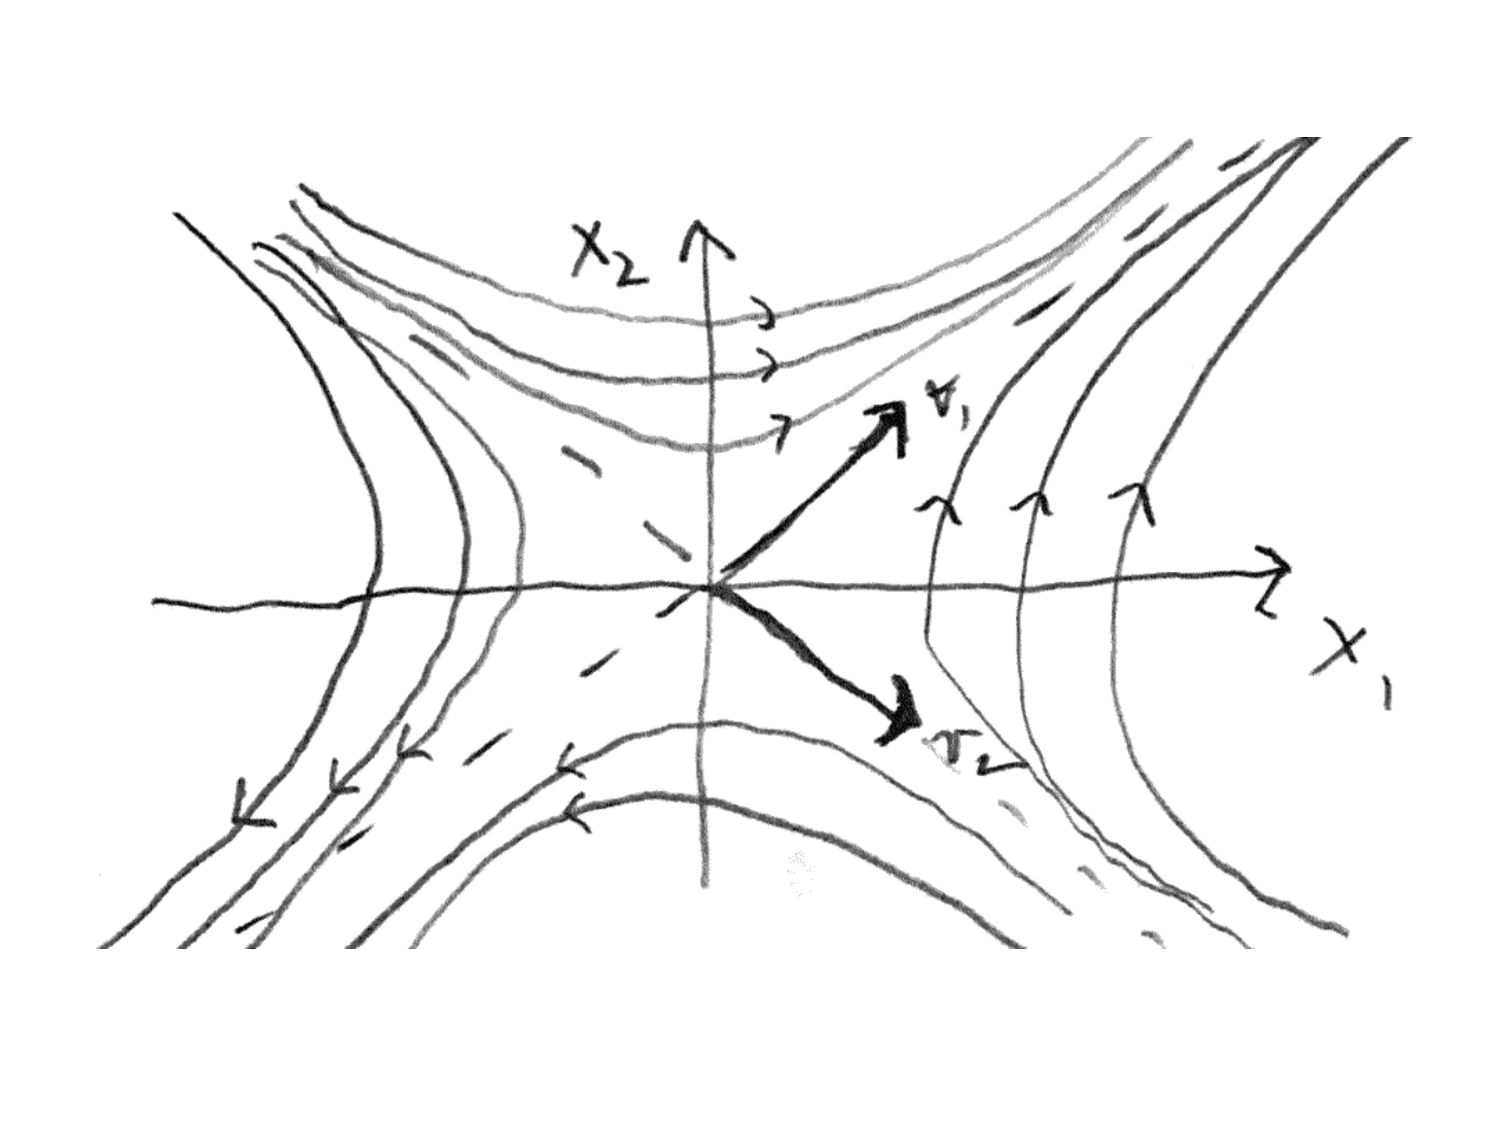
\includegraphics[width=8cm,bb=0 0 10 20]{2019/Midterm1.2019/PhasePortrait4.pdf}
        
        
        % \begin{tikzpicture}[thick,vectorV/.style={-stealth,DarkRed,very thick},
        % curved arrow/.style={arc arrow={to pos #1 with length 2mm and options {}}},
        % reversed curved arrow/.style={arc arrow={to pos #1 with length 2mm and options reversed}}]
        %  \begin{scope}
        %     \draw (-3,0) -- (3,0) node[below] {$x_1$};
        %     \draw (0,-3) -- (0,3) node[left] {$x_2$};
        %     \draw (-120:pi) -- (60:pi) node[pos=0.9,left]{$\lambda_1$ eigenspace};
        %     \draw[vectorV] (0,0) -- (2,2.4) node[right]{$\vec v_1$};
        %     \draw[vectorV] (0,0) -- (2,-0.45) node[below]{$\vec v_2$};
        %     \draw plot [smooth] coordinates { (2.5,-0.3) (0.8,0.2) (2,2)};
        %     \draw plot [smooth] coordinates { (2.5,-0.2) (0.8,0.2) (2,2)};
        %     \end{scope}
        % \end{tikzpicture}

    }    
    \fi
    
 	\newpage\Initials
    \question[4] A tank holds 500 litres of salt water. Initially, there are 0.5 kg of salt in the tank. Salt water containing 3 kg of salt per litre is pumped into the tank at a rate of 4 litres per minute. The well mixed solution is pumped out at a rate of 2 litres per minute. Construct an initial value problem that models the amount of salt in the tank for $t\in[0,T]$, where $T$ is some positive constant. Do not solve your initial value problem. 
    
    \ifnum \sol=0 
    {
    \vspace{5cm}
    }
    \fi
    
    \ifnum \sol=1
    {\color{DarkBlue} \textbf{Solution}\\   
    Let $Q$ be the amount of salt at time $t$. 
    \begin{align*}
        Q'(t) &= \text{(rate in) - (rate out)} \\ 
        &= 3\cdot4 - 2\frac{Q}{500+2t} \\
        &= 12 - \frac{Q}{250+t}, \quad Q(0) = \frac12, \quad t \in [0,T]
    \end{align*}
    }
    \fi
    

    \question[3] Transform the equation $\displaystyle 2y'' + 4 y' + 8ty = 12t^2$ into an equivalent first order system. Express your system in the form $\vec x \, ' = A \vec x + \vec g$, where $\vec x$ and $\vec g$ are vectors in $\mathbb R^2$. 
    \ifnum \sol=0 
    {
    \vspace{4cm}
    }
    \fi    
    
    \ifnum \sol=1
    {\color{DarkBlue} \textbf{Solution}\\ Let 
    \begin{align*}
        x_1 = y , \quad 
        x_2 = y' 
    \end{align*}
    Then 
    \begin{align*}
        x_1' &= x_2 \\
        x_2' &= y'' = 6t^2 - 2x_2 - 4tx_1
    \end{align*}
    As a matrix equation we have
    \begin{align*}
        \vec x \, ' (t) = \spalignmat{x_1';x_2'} = \spalignmat{0 1;-4t -2}\vec x + \spalignmat{0;6t^2}
    \end{align*}
    
    
    }
    \fi
    

    \question[3] % 
    Suppose $\vec x \, ' = A \vec x$, where $A$ is the $2\times 2$ matrix
    $A = \spalignmat{0,-4;4,0}$.
    The eigenvalues of $A$ are $\pm 4i$. Sketch the phase portrait. Label your axes.
    
    
    \newpage\Initials
    \question[10] Consider the differential equation $\displaystyle \dydt = 3y^2 - 2y^3$ where $y=y(t)$ and $t\ge0$.
    \begin{parts}
        \part Indicate the equilibrium solutions.
        \part Sketch the phase line and classify the equilibrium solutions. 
        \part Determine where $y$ is concave up and where it is concave down.
        \part Use the information you obtained in parts (a), (b), and (c) to sketch a few integral curves. 
    
    \end{parts}    
    
    
 	\newpage\Initials    
    
    
    \question[3] An amount $S_0$ is invested at an annual rate of return $r$ percent, compounded continuously. Determine the number of years required for the original investment to double in value, as a function of $r$. 
    
    
    
    \ifnum \sol=0 
    {
    \vspace{4cm}
    }
    \fi    
    \ifnum \sol=1
        {\color{DarkBlue} \textbf{Solution}\\ 
        \textit{Note that this is question 2.3 \# 10. }
        \begin{align*}
            S' &= r S \\ 
            S &= S_0e^{rt} \\
            2S_0 &= S_0e^{rT} \\
            T &= \frac 1r \ln 2
        \end{align*}
    }
    \fi


    
        
    
    \question[4] Consider the system $$ \vec x \, ' = A \vec x = \spalignmat{-1 -4;1 -1} \vec x$$ The eigenvalues of $A$ are $\lambda = -1 \pm 2i$. 
    \begin{enumerate}[label=(\alph*)]
        \item Determine the eigenvectors of $A$. 
        \item Write down the solution to the linear system. 
        \item Classify the critical point(s) of the system in terms of stability and type.
    \end{enumerate}
    
    \ifnum \sol=1
        {\color{DarkBlue} \textbf{Solution}\\ This is based on a question from section 3.4, \# 7. 
    \begin{enumerate}[label=(\alph*)]
        \item The eigenvectors are $\spalignmat{\pm2i;1}=\spalignmat{0;1}+ i\spalignmat{\pm2;0}$.
        \item From the eigenvectors and eigenvalues, we have the solution $$\vec x (t) = e^{-t} \left( \spalignmat{0;1}\cos2t - \spalignmat{2;0 } \sin2t\right) + i e^{-t}\left( \spalignmat{0;1}\sin2t + \spalignmat{2;0 }\cos2t \right)$$
        \item The only critical point is at $(0,0)$ and the critical point is an asymptotically stable spiral sink.
    \end{enumerate}
    
        
        %             \begin{tikzpicture}[thick,
        % curved arrow/.style={arc arrow={to pos #1 with length 2mm and options {}}},
        % reversed curved arrow/.style={arc arrow={to pos #1 with length 2mm and options reversed}}]
        %  \begin{scope}
        %     \draw (-3,0) -- (3,0) node[below] {$x_1$};
        %     \draw (0,-3) -- (0,3) node[left] {$x_2$};
        %     \foreach \X in {2,2.5}
        %     {\draw[rotate=45,curved arrow=0.25] circle (\X cm and 0.4*\X cm);}
        %     \end{scope}
        %     \begin{scope}[xshift=7cm]
        %     \draw (-3,0) -- (3,0) node[below] {$x_1$};
        %     \draw (0,-3) -- (0,3) node[left] {$x_2$};
        %     \draw (-120:pi) -- (60:pi) node[pos=0.9,left]{$v_2$};
        %     \draw[rotate=-20,reversed curved arrow=0.2,curved arrow=0.8]
        %     plot[variable=\x,domain=-1.8:1.8,samples=101] (\x,-\x^3+2*\x);
        %     \draw[rotate=-10,reversed curved arrow=0.2,curved arrow=0.8]
        %     plot[variable=\x,domain=-1.8:1.8,samples=101] (1.5*\x,-\x^3+2*\x);
        %     \end{scope}
        % \end{tikzpicture}
        
        }
    \fi
    

    

    
    
    \newpage\Initials
    \question[2] A small number of points will be allocated for presentation, neatness, and organization. Please ensure that
    \begin{enumerate}
        \item your scan is under 5 MB in file size
        \item your work is legible in the scan
        \item your name or initials are at the top of every page
        \item questions are answered in the order in which they were given
        \item during the upload process you have indicated which pages correspond to which question, and made sure that none of your pages are upside down or sideways (you can also change the orientation of the pages when you upload in Gradescope)
    \end{enumerate}
    Ensuring that these criteria are met helps ensure that your exam is graded efficiently and accurately. 
    
    \question[1] Please sign and date the following GT Honor Code statement. \\ 
    
    \vspace{6pt}
    \textbf{Georgia Tech Honor Code}\\
    \GTHonorCode
    
    \begin{center}
    \begin{center}
        \def\arraystretch{0.35}%  1 is the default, change whatever you need
        \begin{tabular}{ b{8cm} b{8cm} }
        \vspace{.5cm} \underline{\hspace{7cm}} & \vspace{.5cm} \underline{\hspace{4.5cm}}  \tabularnewline
        \vspace{6pt} signature & \vspace{6pt} date    
        \end{tabular}
    \end{center}
    \end{center}

\end{questions}



\end{document}


